\title[Short title]{Processing Seismic Data in the Presence of Residual Statics}
\author{Aaron Stanton, Nasser Kazemi, and Mauricio D. Sacchi}
\institute{Signal Analysis and Imaging Group \\ Department of Physics \\ University of Alberta}
\date{}

\addtobeamertemplate{frametitle}{}{%
\begin{textblock*}{100mm}(.85\textwidth,-0.9cm)
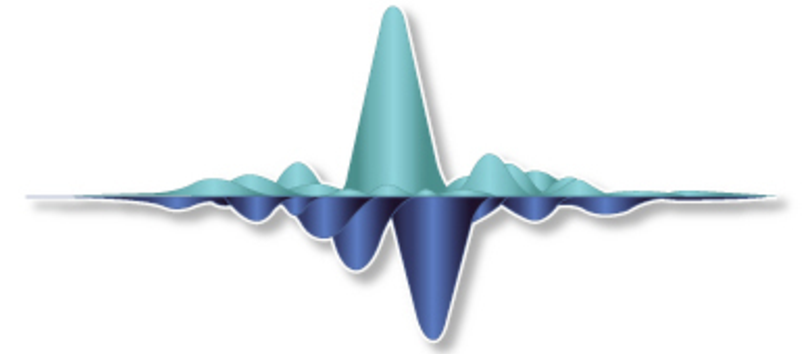
\includegraphics[height=1cm,width=2cm]{logo}
\end{textblock*}}

\maketitle



\begin{frame} \frametitle{Outline}
    \begin{itemize}
        \item Motivation
        \item Algorithm
        \item Synthetic Examples
        \item Real Examples
    \end{itemize}
\end{frame}

\begin{frame} \frametitle{Motivation}
    \begin{itemize}
        \item Here's a bullet.
        \item And another bullet.
        \item and one more.
    \end{itemize}
    \pause
    \begin{itemize}
        \item Another set of bullets.
            \pause
        \item But these are hidden from one another.
            \pause
        \item Which can be used to make animations.
    \end{itemize}
\end{frame}

\begin{frame} \frametitle{Algorithm}
    \Huge{$\nabla^2 u - \alpha \frac{\partial u}{\partial t} = \delta(\mathbf{x},t)$}
\end{frame}

\inputdir{syn5d}
% we could also use includegraphics here instead
\begin{frame} \frametitle{Plots}
    \plot{data1}{width=0.45\textwidth}{}
\end{frame}

\begin{frame} \frametitle{Multiplots}
    \multiplot{2}{data1,data1}{width=0.45\textwidth}{}
\end{frame}
